\documentclass[a4paper,12pt]{article}
\usepackage[margin=18mm]{geometry}
\usepackage{tikz}
\usepackage{amsmath}
\newcommand{\pFourCell}[2]{\makebox[#1em][c]{\ensuremath{#2}}}
\pagestyle{empty}
\begin{document}
\section*{Spaltentreue LaTeX-Ausgabe}
\noindent Gleichung: \texttt{2*sqrt((x+3)/(2+1))=5} \hfill Zielvariable: \texttt{x} \hfill Profil: \texttt{standard}

\vspace{8mm}
\begin{center}
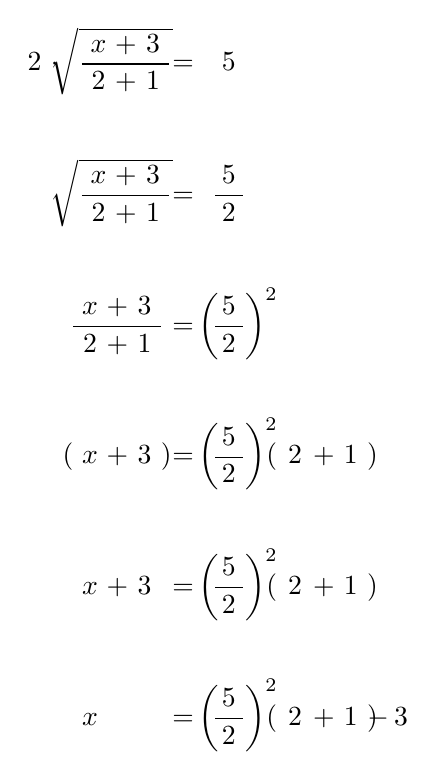
\begin{tikzpicture}[x=1em,y=-1em]
\node[anchor=base, inner sep=0pt] at (0.44,2.9) {$2$};
\node[anchor=base, inner sep=0pt] at (1.17,2.9) {$\cdot$};
\node[anchor=base, inner sep=0pt] at (3.23,2.9) {$\pFourCell{3.54}{\sqrt{\displaystyle\frac{\pFourCell{1.2}{x}\pFourCell{0.78}{+}\pFourCell{1.18}{3}}{\pFourCell{1.2}{2}\pFourCell{0.78}{+}\pFourCell{1.18}{1}}}}$};
\node[anchor=base, inner sep=0pt] at (5.81,2.9) {$=$};
\node[anchor=base, inner sep=0pt] at (7.46,2.9) {$5$};
\node[anchor=base, inner sep=0pt] at (7.46,7.65) {$\displaystyle\frac{\pFourCell{1}{5}}{\pFourCell{1}{2}}$};
\node[anchor=base, inner sep=0pt] at (3.23,7.65) {$\pFourCell{3.54}{\sqrt{\displaystyle\frac{\pFourCell{1.2}{x}\pFourCell{0.78}{+}\pFourCell{1.18}{3}}{\pFourCell{1.2}{2}\pFourCell{0.78}{+}\pFourCell{1.18}{1}}}}$};
\node[anchor=base, inner sep=0pt] at (5.81,7.65) {$=$};
\node[anchor=base, inner sep=0pt] at (3.42,12.385) {$\displaystyle\frac{\pFourCell{1.2}{x}\pFourCell{0.78}{+}\pFourCell{1.18}{3}}{\pFourCell{1.2}{2}\pFourCell{0.78}{+}\pFourCell{1.18}{1}}$};
\node[anchor=base, inner sep=0pt] at (5.81,12.385) {$=$};
\node[anchor=base, inner sep=0pt] at (7.46,12.385) {$\displaystyle\frac{\pFourCell{1}{5}}{\pFourCell{1}{2}}$};
\node[anchor=base, inner sep=0pt] at (6.79,12.385) {$\pFourCell{0.34}{\left(\vphantom{\displaystyle\frac{\pFourCell{1}{5}}{\pFourCell{1}{2}}}\right.}$};
\node[anchor=base, inner sep=0pt] at (8.58,12.385) {$\pFourCell{1.24}{\left.\vphantom{\displaystyle\frac{\pFourCell{1}{5}}{\pFourCell{1}{2}}}\right)^{2}}$};
\node[anchor=base, inner sep=0pt] at (3.42,17.105) {$\left(\pFourCell{1.2}{x}\pFourCell{0.78}{+}\pFourCell{1.18}{3}\right)$};
\node[anchor=base, inner sep=0pt] at (5.81,17.105) {$=$};
\node[anchor=base, inner sep=0pt] at (7.46,17.105) {$\displaystyle\frac{\pFourCell{1}{5}}{\pFourCell{1}{2}}$};
\node[anchor=base, inner sep=0pt] at (6.79,17.105) {$\pFourCell{0.34}{\left(\vphantom{\displaystyle\frac{\pFourCell{1}{5}}{\pFourCell{1}{2}}}\right.}$};
\node[anchor=base, inner sep=0pt] at (8.58,17.105) {$\pFourCell{1.24}{\left.\vphantom{\displaystyle\frac{\pFourCell{1}{5}}{\pFourCell{1}{2}}}\right)^{2}}$};
\node[anchor=base, inner sep=0pt] at (10.83,17.105) {$\left(\pFourCell{1.3}{2}\pFourCell{0.78}{+}\pFourCell{1.18}{1}\right)$};
\node[anchor=base, inner sep=0pt] at (2.44,21.825) {$x$};
\node[anchor=base, inner sep=0pt] at (3.43,21.825) {$+$};
\node[anchor=base, inner sep=0pt] at (4.41,21.825) {$3$};
\node[anchor=base, inner sep=0pt] at (5.81,21.825) {$=$};
\node[anchor=base, inner sep=0pt] at (7.46,21.825) {$\displaystyle\frac{\pFourCell{1}{5}}{\pFourCell{1}{2}}$};
\node[anchor=base, inner sep=0pt] at (6.79,21.825) {$\pFourCell{0.34}{\left(\vphantom{\displaystyle\frac{\pFourCell{1}{5}}{\pFourCell{1}{2}}}\right.}$};
\node[anchor=base, inner sep=0pt] at (8.58,21.825) {$\pFourCell{1.24}{\left.\vphantom{\displaystyle\frac{\pFourCell{1}{5}}{\pFourCell{1}{2}}}\right)^{2}}$};
\node[anchor=base, inner sep=0pt] at (10.83,21.825) {$\left(\pFourCell{1.3}{2}\pFourCell{0.78}{+}\pFourCell{1.18}{1}\right)$};
\node[anchor=base, inner sep=0pt] at (2.44,26.545) {$x$};
\node[anchor=base, inner sep=0pt] at (5.81,26.545) {$=$};
\node[anchor=base, inner sep=0pt] at (7.46,26.545) {$\displaystyle\frac{\pFourCell{1}{5}}{\pFourCell{1}{2}}$};
\node[anchor=base, inner sep=0pt] at (6.79,26.545) {$\pFourCell{0.34}{\left(\vphantom{\displaystyle\frac{\pFourCell{1}{5}}{\pFourCell{1}{2}}}\right.}$};
\node[anchor=base, inner sep=0pt] at (8.58,26.545) {$\pFourCell{1.24}{\left.\vphantom{\displaystyle\frac{\pFourCell{1}{5}}{\pFourCell{1}{2}}}\right)^{2}}$};
\node[anchor=base, inner sep=0pt] at (10.83,26.545) {$\left(\pFourCell{1.3}{2}\pFourCell{0.78}{+}\pFourCell{1.18}{1}\right)$};
\node[anchor=base, inner sep=0pt] at (12.85,26.545) {$-$};
\node[anchor=base, inner sep=0pt] at (13.68,26.545) {$3$};
\end{tikzpicture}
\end{center}

\newpage
\section*{Spaltentreue LaTeX-Ausgabe mit Spaltengrenzen}
\vspace{6mm}
\begin{center}
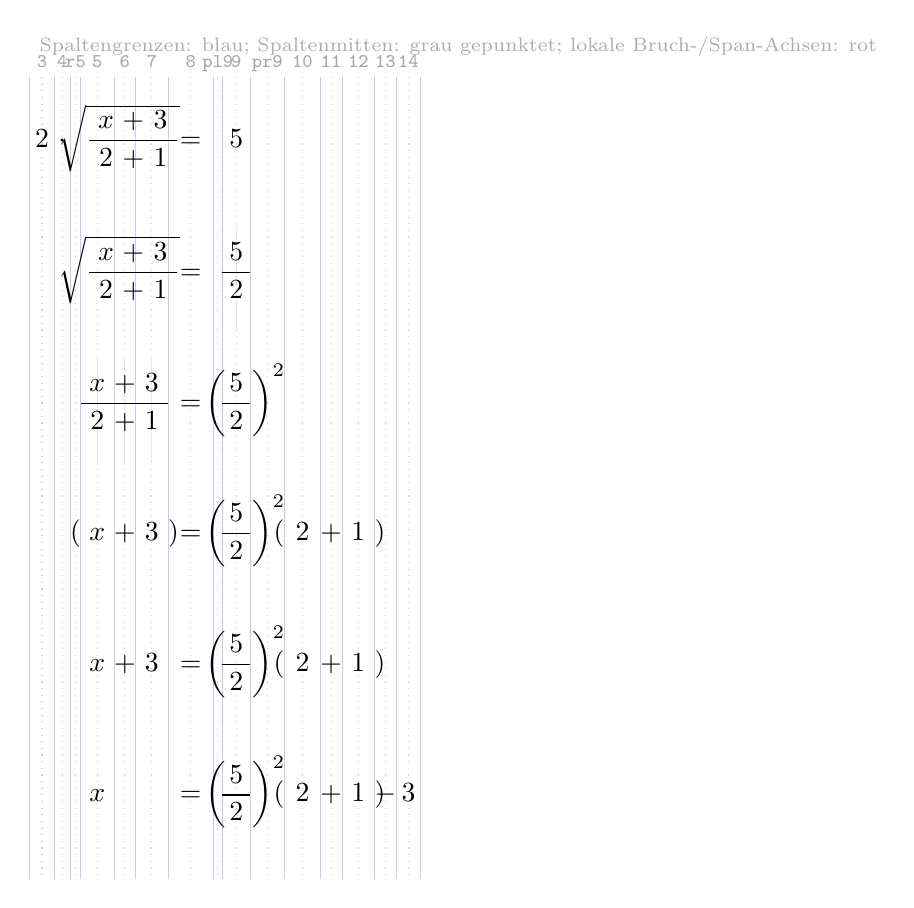
\begin{tikzpicture}[x=1em,y=-1em]
\node[font={\scriptsize}, text=gray!65, anchor=west] at (0,-0.75) {Spaltengrenzen: blau; Spaltenmitten: grau gepunktet; lokale Bruch-/Span-Achsen: rot};
\draw[blue!22, line width=0.28pt] (0,0.35) -- (0,29.33);
\draw[blue!22, line width=0.28pt] (0.88,0.35) -- (0.88,29.33);
\draw[blue!22, line width=0.28pt] (1.46,0.35) -- (1.46,29.33);
\draw[blue!22, line width=0.28pt] (1.84,0.35) -- (1.84,29.33);
\draw[blue!22, line width=0.28pt] (3.04,0.35) -- (3.04,29.33);
\draw[blue!22, line width=0.28pt] (3.82,0.35) -- (3.82,29.33);
\draw[blue!22, line width=0.28pt] (5,0.35) -- (5,29.33);
\draw[blue!22, line width=0.28pt] (6.62,0.35) -- (6.62,29.33);
\draw[blue!22, line width=0.28pt] (6.96,0.35) -- (6.96,29.33);
\draw[blue!22, line width=0.28pt] (7.96,0.35) -- (7.96,29.33);
\draw[blue!22, line width=0.28pt] (9.2,0.35) -- (9.2,29.33);
\draw[blue!22, line width=0.28pt] (10.5,0.35) -- (10.5,29.33);
\draw[blue!22, line width=0.28pt] (11.28,0.35) -- (11.28,29.33);
\draw[blue!22, line width=0.28pt] (12.46,0.35) -- (12.46,29.33);
\draw[blue!22, line width=0.28pt] (13.24,0.35) -- (13.24,29.33);
\draw[blue!22, line width=0.28pt] (14.12,0.35) -- (14.12,29.33);
\draw[gray!35, dotted] (0.44,0.35) -- (0.44,29.33);
\node[font={\ttfamily\scriptsize}, text=gray!70, anchor=base] at (0.44,0) {3};
\draw[gray!35, dotted] (1.17,0.35) -- (1.17,29.33);
\node[font={\ttfamily\scriptsize}, text=gray!70, anchor=base] at (1.17,0) {4};
\draw[gray!35, dotted] (1.65,0.35) -- (1.65,29.33);
\node[font={\ttfamily\scriptsize}, text=gray!70, anchor=base] at (1.65,0) {r5};
\draw[gray!35, dotted] (2.44,0.35) -- (2.44,29.33);
\node[font={\ttfamily\scriptsize}, text=gray!70, anchor=base] at (2.44,0) {5};
\draw[gray!35, dotted] (3.43,0.35) -- (3.43,29.33);
\node[font={\ttfamily\scriptsize}, text=gray!70, anchor=base] at (3.43,0) {6};
\draw[gray!35, dotted] (4.41,0.35) -- (4.41,29.33);
\node[font={\ttfamily\scriptsize}, text=gray!70, anchor=base] at (4.41,0) {7};
\draw[gray!35, dotted] (5.81,0.35) -- (5.81,29.33);
\node[font={\ttfamily\scriptsize}, text=gray!70, anchor=base] at (5.81,0) {8};
\draw[gray!35, dotted] (6.79,0.35) -- (6.79,29.33);
\node[font={\ttfamily\scriptsize}, text=gray!70, anchor=base] at (6.79,0) {pl9};
\draw[gray!35, dotted] (7.46,0.35) -- (7.46,29.33);
\node[font={\ttfamily\scriptsize}, text=gray!70, anchor=base] at (7.46,0) {9};
\draw[gray!35, dotted] (8.58,0.35) -- (8.58,29.33);
\node[font={\ttfamily\scriptsize}, text=gray!70, anchor=base] at (8.58,0) {pr9};
\draw[gray!35, dotted] (9.85,0.35) -- (9.85,29.33);
\node[font={\ttfamily\scriptsize}, text=gray!70, anchor=base] at (9.85,0) {10};
\draw[gray!35, dotted] (10.89,0.35) -- (10.89,29.33);
\node[font={\ttfamily\scriptsize}, text=gray!70, anchor=base] at (10.89,0) {11};
\draw[gray!35, dotted] (11.87,0.35) -- (11.87,29.33);
\node[font={\ttfamily\scriptsize}, text=gray!70, anchor=base] at (11.87,0) {12};
\draw[gray!35, dotted] (12.85,0.35) -- (12.85,29.33);
\node[font={\ttfamily\scriptsize}, text=gray!70, anchor=base] at (12.85,0) {13};
\draw[gray!35, dotted] (13.68,0.35) -- (13.68,29.33);
\node[font={\ttfamily\scriptsize}, text=gray!70, anchor=base] at (13.68,0) {14};
\node[anchor=base, inner sep=0pt] at (0.44,2.9) {$2$};
\node[anchor=base, inner sep=0pt] at (1.17,2.9) {$\cdot$};
\node[anchor=base, inner sep=0pt] at (3.23,2.9) {$\pFourCell{3.54}{\sqrt{\displaystyle\frac{\pFourCell{1.2}{x}\pFourCell{0.78}{+}\pFourCell{1.18}{3}}{\pFourCell{1.2}{2}\pFourCell{0.78}{+}\pFourCell{1.18}{1}}}}$};
\node[anchor=base, inner sep=0pt] at (5.81,2.9) {$=$};
\node[anchor=base, inner sep=0pt] at (7.46,2.9) {$5$};
\draw[red!30, opacity=0.32, line width=0.35pt] (7.46,5.75) -- (7.46,9.55);
\node[anchor=base, inner sep=0pt] at (7.46,7.65) {$\displaystyle\frac{\pFourCell{1}{5}}{\pFourCell{1}{2}}$};
\node[anchor=base, inner sep=0pt] at (3.23,7.65) {$\pFourCell{3.54}{\sqrt{\displaystyle\frac{\pFourCell{1.2}{x}\pFourCell{0.78}{+}\pFourCell{1.18}{3}}{\pFourCell{1.2}{2}\pFourCell{0.78}{+}\pFourCell{1.18}{1}}}}$};
\node[anchor=base, inner sep=0pt] at (5.81,7.65) {$=$};
\draw[red!30, opacity=0.32, line width=0.35pt] (2.44,10.5) -- (2.44,14.27);
\draw[red!30, opacity=0.32, line width=0.35pt] (3.43,10.5) -- (3.43,14.27);
\draw[red!30, opacity=0.32, line width=0.35pt] (4.41,10.5) -- (4.41,14.27);
\node[anchor=base, inner sep=0pt] at (3.42,12.385) {$\displaystyle\frac{\pFourCell{1.2}{x}\pFourCell{0.78}{+}\pFourCell{1.18}{3}}{\pFourCell{1.2}{2}\pFourCell{0.78}{+}\pFourCell{1.18}{1}}$};
\node[anchor=base, inner sep=0pt] at (5.81,12.385) {$=$};
\node[anchor=base, inner sep=0pt] at (7.46,12.385) {$\displaystyle\frac{\pFourCell{1}{5}}{\pFourCell{1}{2}}$};
\node[anchor=base, inner sep=0pt] at (6.79,12.385) {$\pFourCell{0.34}{\left(\vphantom{\displaystyle\frac{\pFourCell{1}{5}}{\pFourCell{1}{2}}}\right.}$};
\node[anchor=base, inner sep=0pt] at (8.58,12.385) {$\pFourCell{1.24}{\left.\vphantom{\displaystyle\frac{\pFourCell{1}{5}}{\pFourCell{1}{2}}}\right)^{2}}$};
\node[anchor=base, inner sep=0pt] at (3.42,17.105) {$\left(\pFourCell{1.2}{x}\pFourCell{0.78}{+}\pFourCell{1.18}{3}\right)$};
\node[anchor=base, inner sep=0pt] at (5.81,17.105) {$=$};
\node[anchor=base, inner sep=0pt] at (7.46,17.105) {$\displaystyle\frac{\pFourCell{1}{5}}{\pFourCell{1}{2}}$};
\node[anchor=base, inner sep=0pt] at (6.79,17.105) {$\pFourCell{0.34}{\left(\vphantom{\displaystyle\frac{\pFourCell{1}{5}}{\pFourCell{1}{2}}}\right.}$};
\node[anchor=base, inner sep=0pt] at (8.58,17.105) {$\pFourCell{1.24}{\left.\vphantom{\displaystyle\frac{\pFourCell{1}{5}}{\pFourCell{1}{2}}}\right)^{2}}$};
\node[anchor=base, inner sep=0pt] at (10.83,17.105) {$\left(\pFourCell{1.3}{2}\pFourCell{0.78}{+}\pFourCell{1.18}{1}\right)$};
\node[anchor=base, inner sep=0pt] at (2.44,21.825) {$x$};
\node[anchor=base, inner sep=0pt] at (3.43,21.825) {$+$};
\node[anchor=base, inner sep=0pt] at (4.41,21.825) {$3$};
\node[anchor=base, inner sep=0pt] at (5.81,21.825) {$=$};
\node[anchor=base, inner sep=0pt] at (7.46,21.825) {$\displaystyle\frac{\pFourCell{1}{5}}{\pFourCell{1}{2}}$};
\node[anchor=base, inner sep=0pt] at (6.79,21.825) {$\pFourCell{0.34}{\left(\vphantom{\displaystyle\frac{\pFourCell{1}{5}}{\pFourCell{1}{2}}}\right.}$};
\node[anchor=base, inner sep=0pt] at (8.58,21.825) {$\pFourCell{1.24}{\left.\vphantom{\displaystyle\frac{\pFourCell{1}{5}}{\pFourCell{1}{2}}}\right)^{2}}$};
\node[anchor=base, inner sep=0pt] at (10.83,21.825) {$\left(\pFourCell{1.3}{2}\pFourCell{0.78}{+}\pFourCell{1.18}{1}\right)$};
\node[anchor=base, inner sep=0pt] at (2.44,26.545) {$x$};
\node[anchor=base, inner sep=0pt] at (5.81,26.545) {$=$};
\node[anchor=base, inner sep=0pt] at (7.46,26.545) {$\displaystyle\frac{\pFourCell{1}{5}}{\pFourCell{1}{2}}$};
\node[anchor=base, inner sep=0pt] at (6.79,26.545) {$\pFourCell{0.34}{\left(\vphantom{\displaystyle\frac{\pFourCell{1}{5}}{\pFourCell{1}{2}}}\right.}$};
\node[anchor=base, inner sep=0pt] at (8.58,26.545) {$\pFourCell{1.24}{\left.\vphantom{\displaystyle\frac{\pFourCell{1}{5}}{\pFourCell{1}{2}}}\right)^{2}}$};
\node[anchor=base, inner sep=0pt] at (10.83,26.545) {$\left(\pFourCell{1.3}{2}\pFourCell{0.78}{+}\pFourCell{1.18}{1}\right)$};
\node[anchor=base, inner sep=0pt] at (12.85,26.545) {$-$};
\node[anchor=base, inner sep=0pt] at (13.68,26.545) {$3$};
\end{tikzpicture}
\end{center}
\end{document}
